\documentclass{article}
\usepackage{amssymb}
\usepackage{amsmath}
\usepackage{graphicx}
\usepackage{subfigure}
\usepackage{float}
\usepackage[margin=1in]{geometry}
\author{Tianyu Dai, Xiaoqing Li, Yuheng Liao, Xuejian Ma}
\title{PHY566 - Percolation}
\begin{document}
\date{4/12/2017}
\maketitle
Percolation theory describes the behavior of connected cluster in a random graph. It usually concerns the movement and filtering of fluids through porous materials. In this project, we simulate the percolation transition and try to analyze its properties.
\section{Determine the critical probability $p_c$}
The basic idea to simulate the percolation transition is to take a $N\times N$ lattice, and then occupy the lattice sites at random according to a certain probability $p$. If a cluster of occupied sites spans the entire lattice from edge to edge, it's called a spanning cluster. The probability of the appearance of a spanning cluster rises with the rise of $p$. When $p$ is relatively small, it is highly unlikely to get a spanning cluster. However, for $p$ large enough, the existence of spanning cluster is guaranteed. The transition from one regime to the other is rather sharp and occurs at a critical concentration, which we call $p_c$. For $N\times N$ lattice, our basic task is to simulate the percolation transitions with different probability $p$, and figure out the $p_c$. Doing those for different $N$, and then plot $p_c - N^{-1}$ graph. From $p_c(N^{-1})$ graph, we can extrapolate to the infinite size limit $p_c(0)$.\\
\indent The program details we should follow for $N\times N$ lattice is as below:\\
\begin{enumerate}
\item Begin with an empty $N\times N$ lattice and initialize all sites to zero, i.e. unoccupied.
\item Select and occupy a random site, labeling it with a cluster number of 1, since it is the first cluster.
\item Select another site at random and check neighboring sites to see if any belongs to a cluster created before. If not, the new site should be labeled with the next cluster number (here, it's number 2). If so, we need to discuss among the following two situations:

\begin{enumerate}
\item If there's only one cluster number among all neighboring sites, give this number to the new site.
\item If there are several cluster number among all occupied neighbors, the new site is considered as a site bridge which connects multiple clusters into one. We should choose a common unique cluster number for resulting cluster, and then also give this number to the new site and relabel all sites in merged cluster to that number.
\end{enumerate}

\item Repeat step 3 until a common cluster number appears on all edges of the lattice.
\item The common cluster number is the number of the spanning cluster, and the fraction of all occupied sites among all lattice sites is $p_c$
\end{enumerate}

Following the steps above, we can get the spanning clusters for different $N\in\{5, 10, 15, 20, 30, 50, 80\}$ as below:

\begin{figure}[H]%[!htb]

\minipage{0.5\textwidth}
  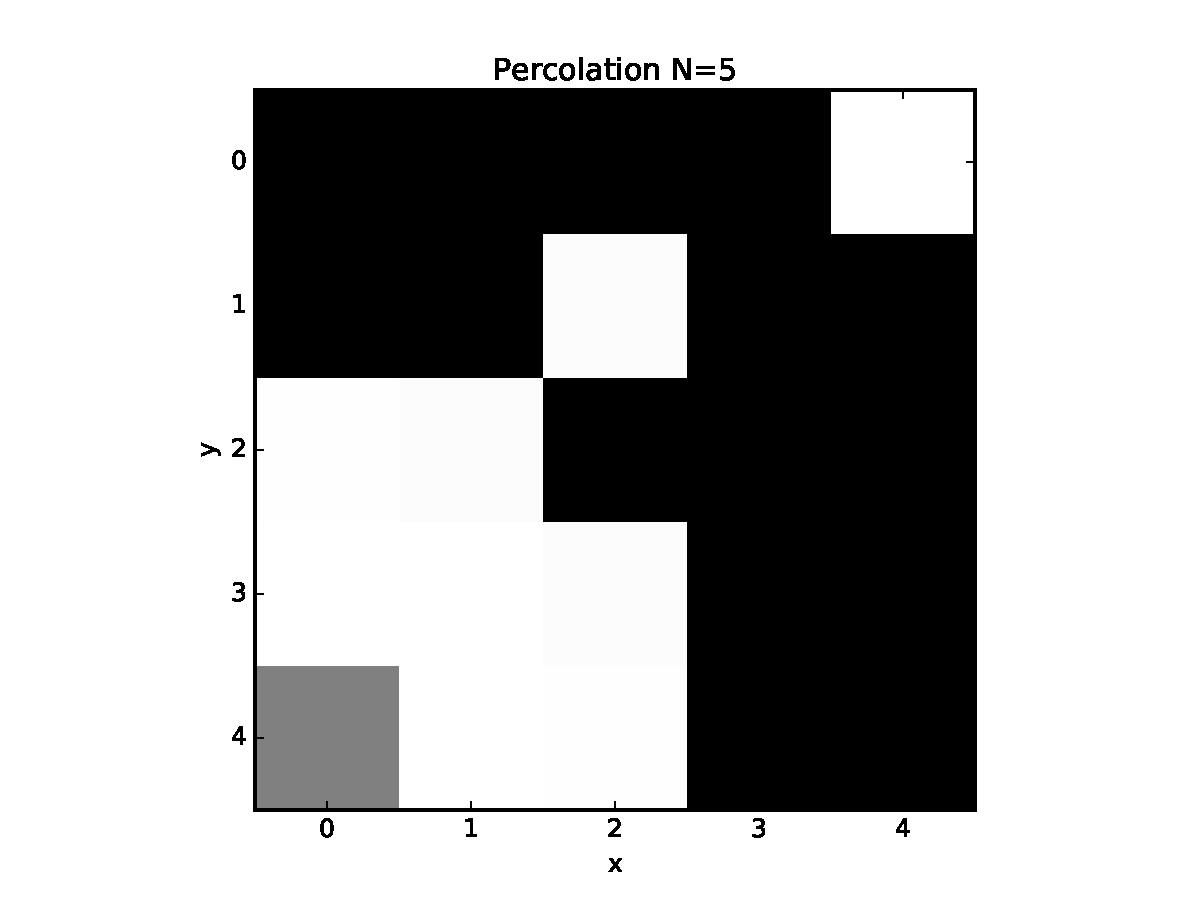
\includegraphics[width=\linewidth]{percolation_5.pdf}
  \label{delta02}
\endminipage\hfill
\minipage{0.5\textwidth}
  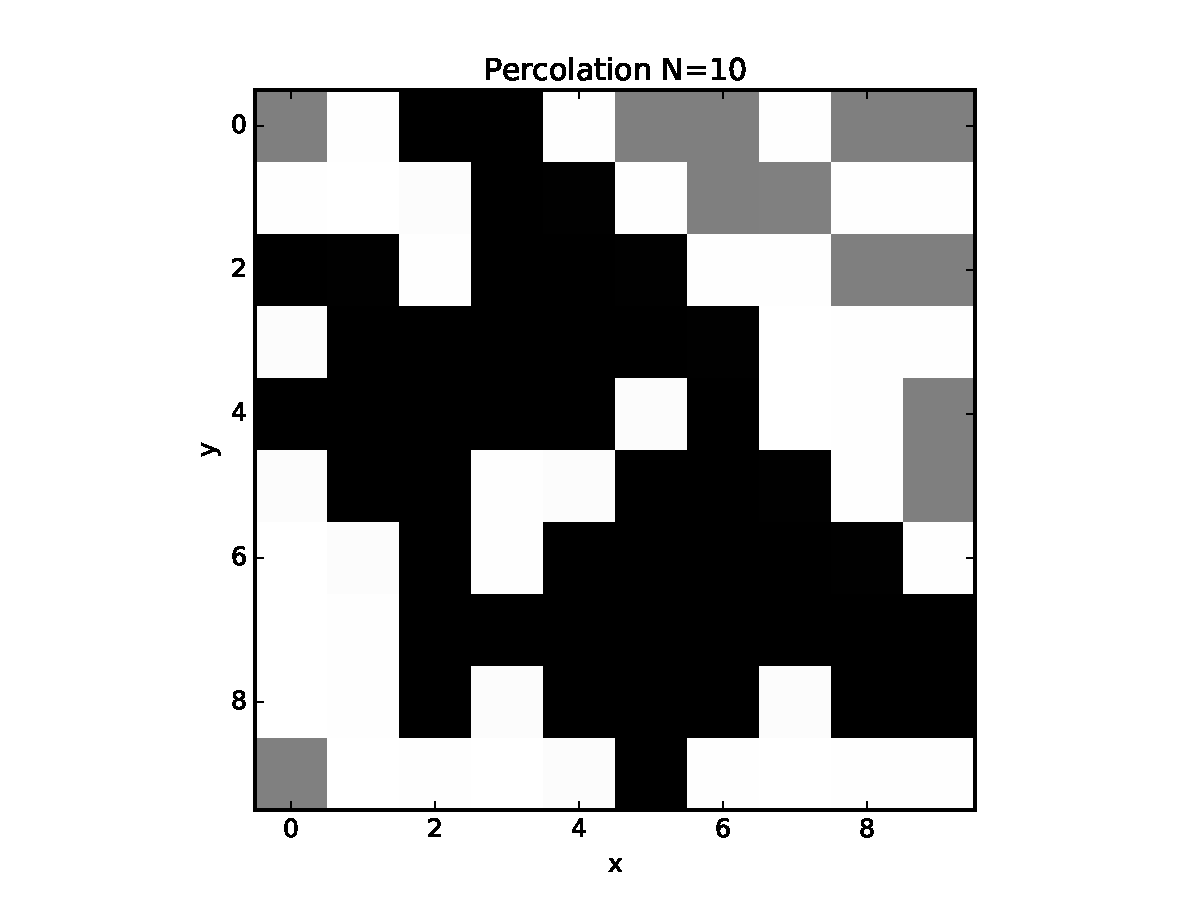
\includegraphics[width=\linewidth]{percolation_10.pdf}
  \label{delta02}
\endminipage\hfill
\minipage{0.5\textwidth}
  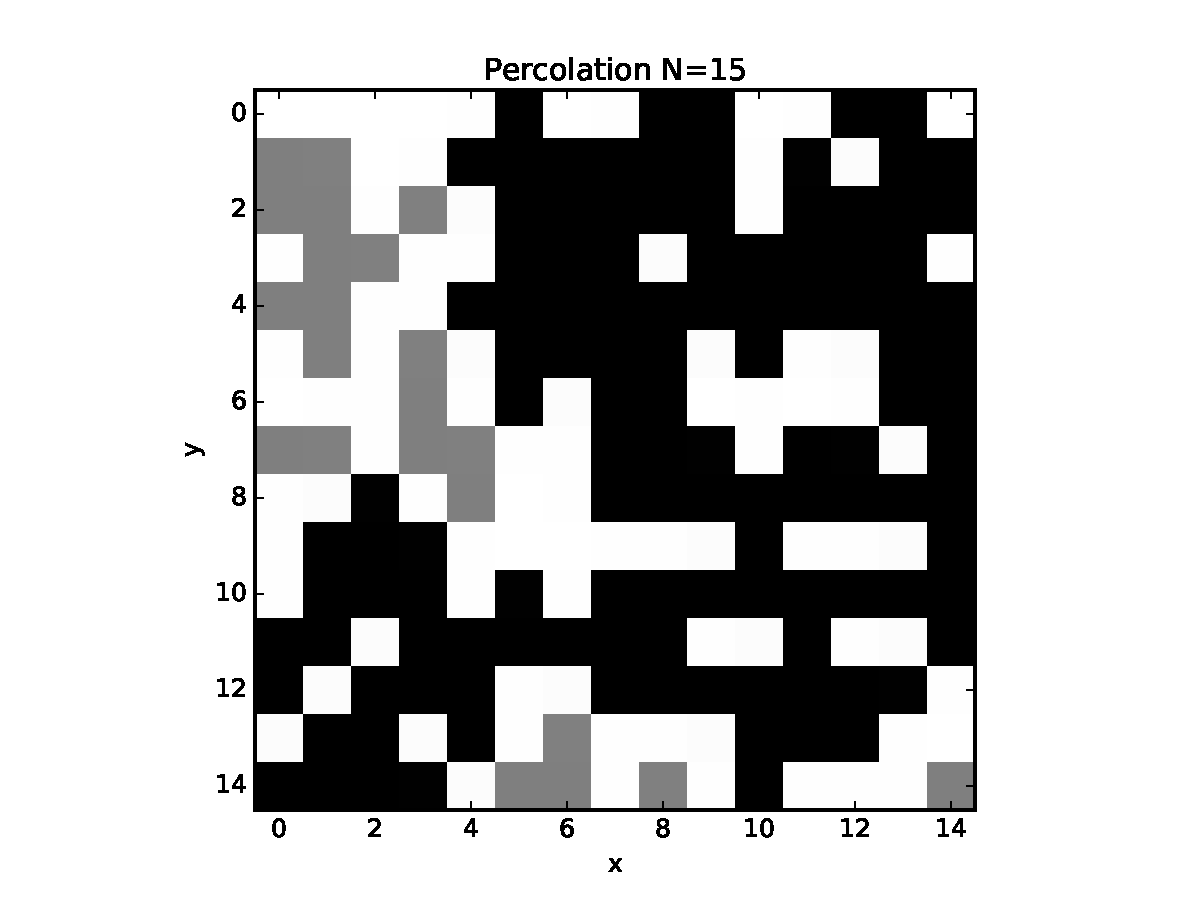
\includegraphics[width=\linewidth]{percolation_15.pdf}
  \label{delta02}
\endminipage\hfill
\minipage{0.5\textwidth}
  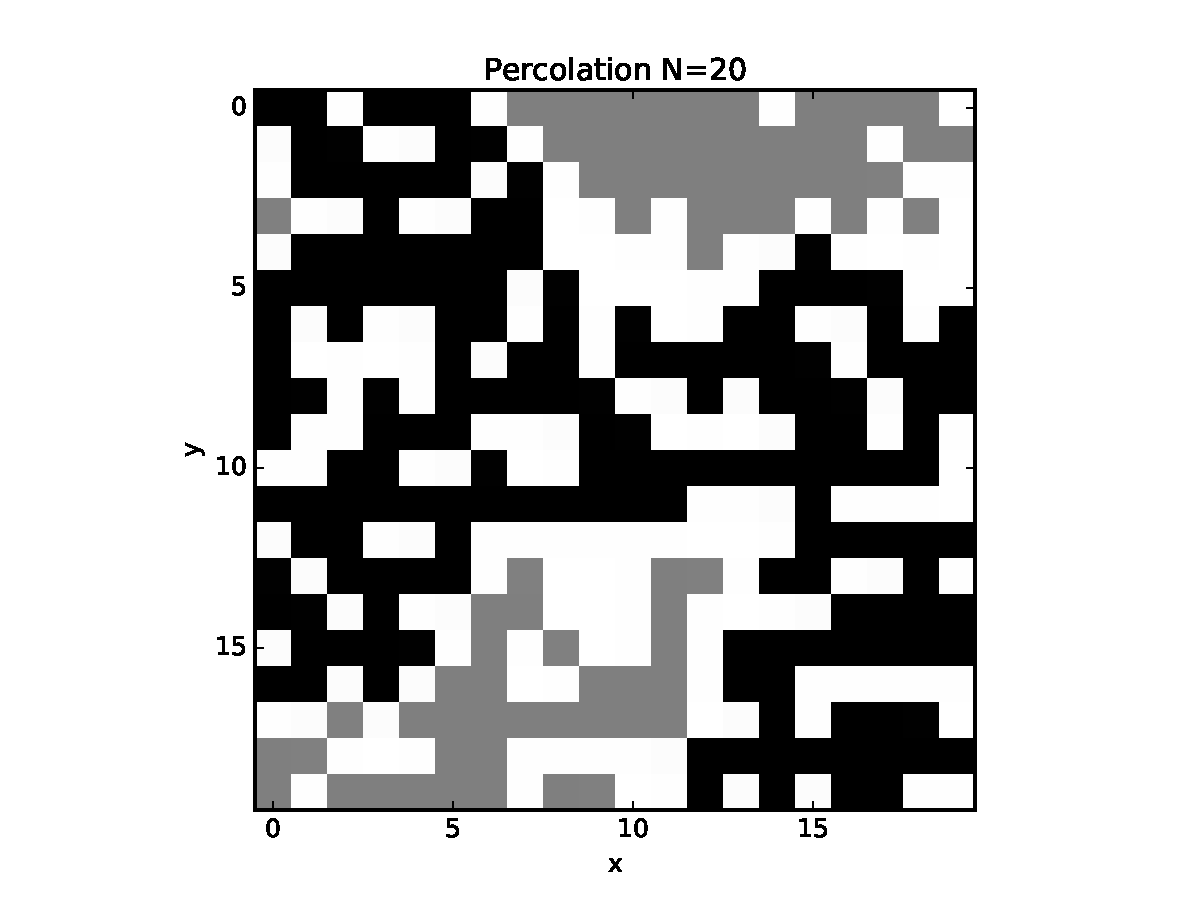
\includegraphics[width=\linewidth]{percolation_20.pdf}
  \label{delta02}
\endminipage\hfill
\minipage{0.5\textwidth}
  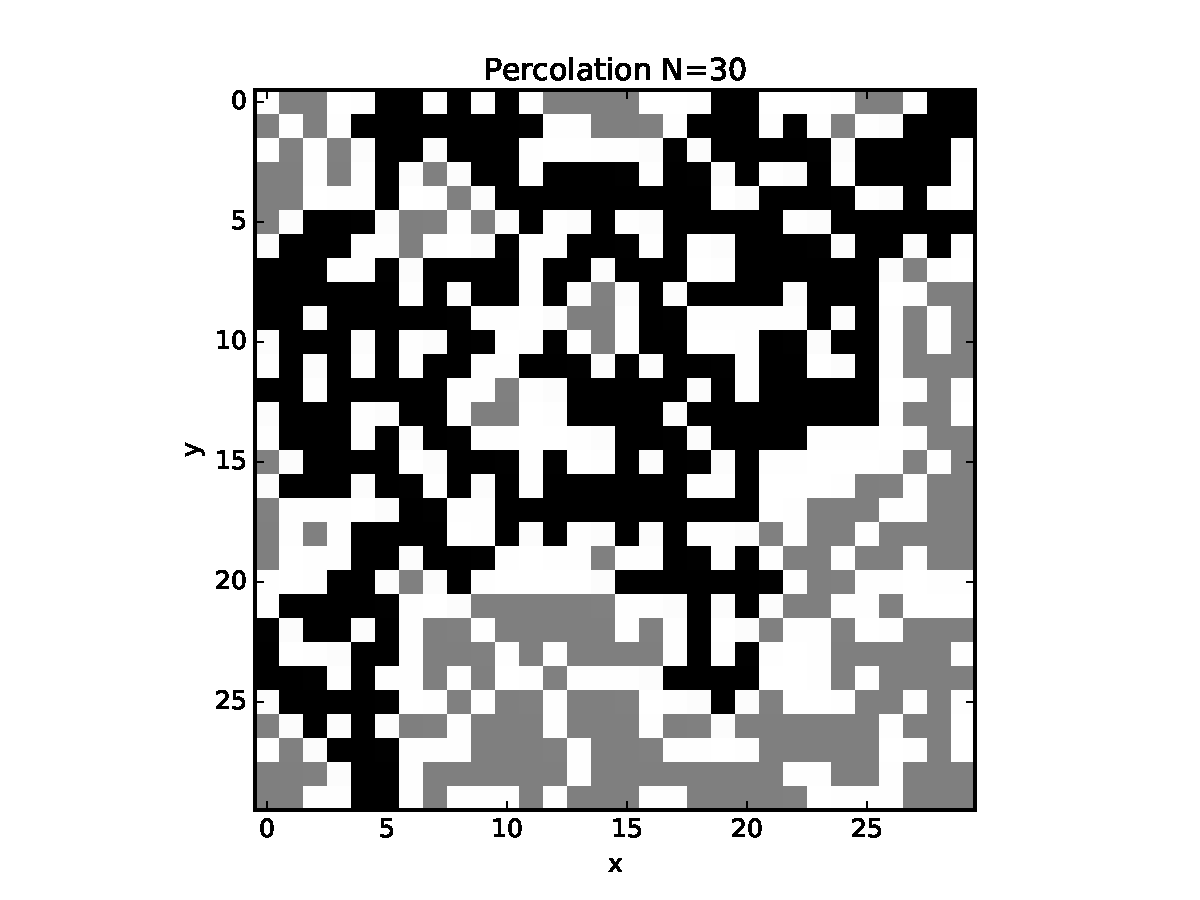
\includegraphics[width=\linewidth]{percolation_30.pdf}
  \label{delta02}
\endminipage\hfill
\minipage{0.5\textwidth}
  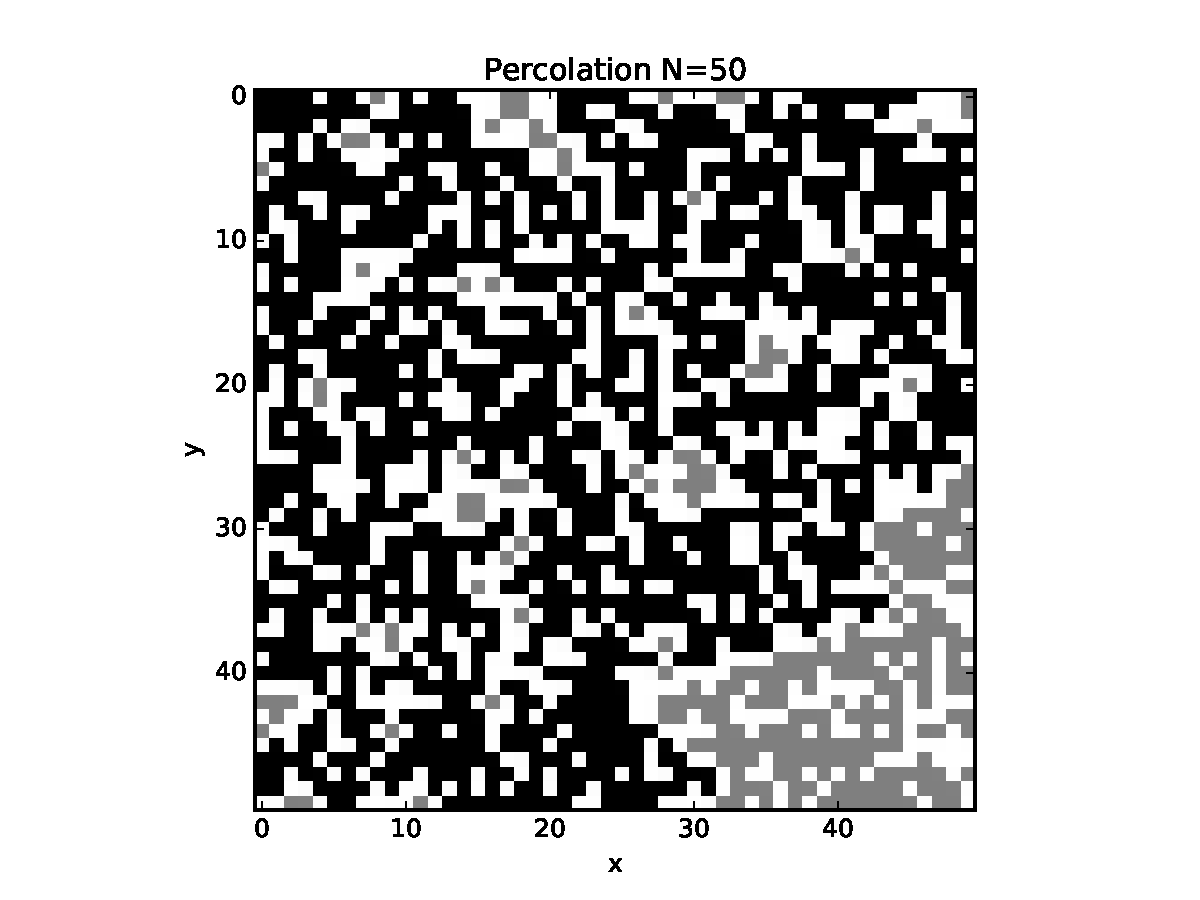
\includegraphics[width=\linewidth]{percolation_50.pdf}
  \label{delta02}
\endminipage\hfill
\end{figure}
\begin{figure}[H]
\minipage{0.5\textwidth}
  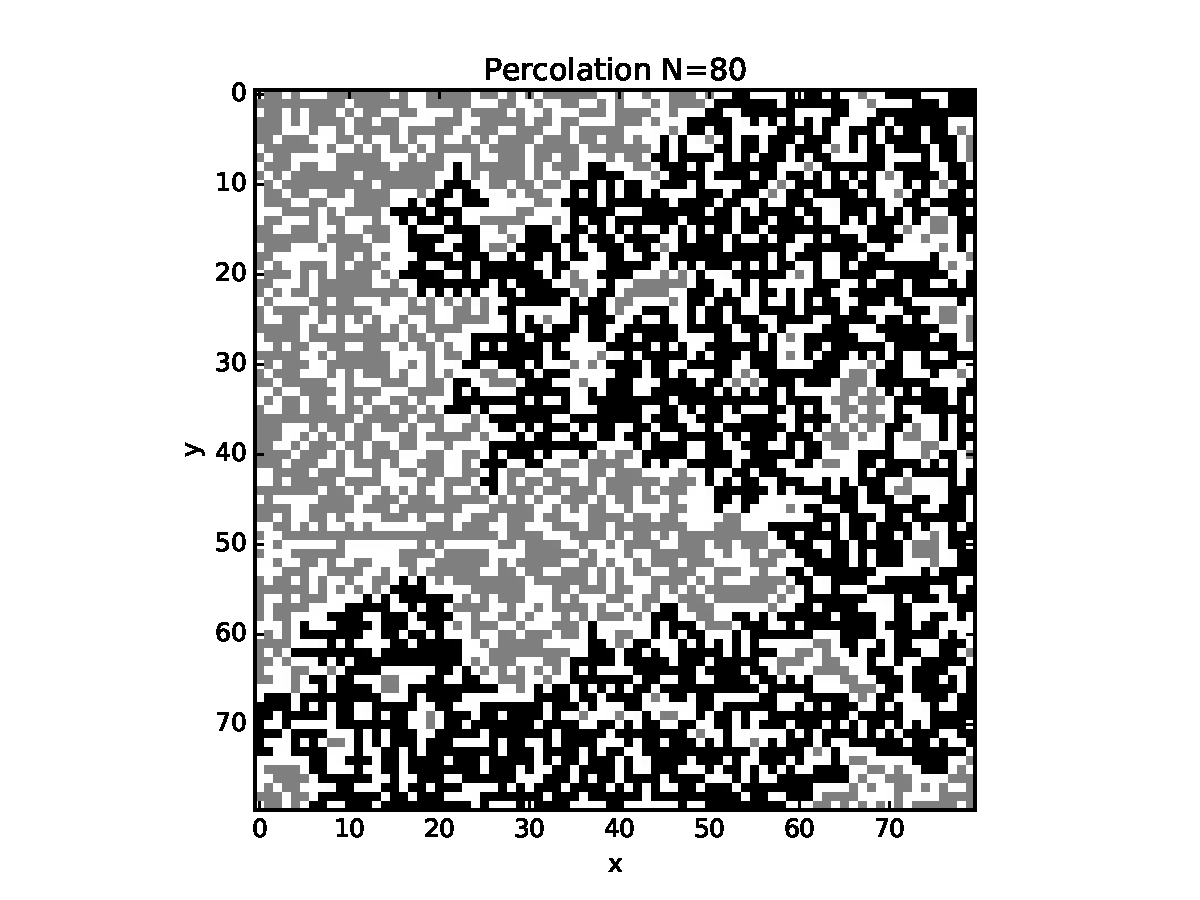
\includegraphics[width=\linewidth]{percolation_80.pdf}
  \label{delta02}
\endminipage\hfill
\end{figure}
In the pictures above, black sites represent sites of spanning clusters, gray ones represent sites occupied while not belonging to spanning clusters, and white ones represent sites unoccupied.\\
\indent By repeating the procedures over 50 times for each $N$, we can calculate the average $p_c(N^{-1})$. After doing so for all $N\in\{5, 10, 15, 20, 30, 50, 80\}$, we could pplot the graph of $p_c(N^{-1})$ as below:
\begin{figure}[H]
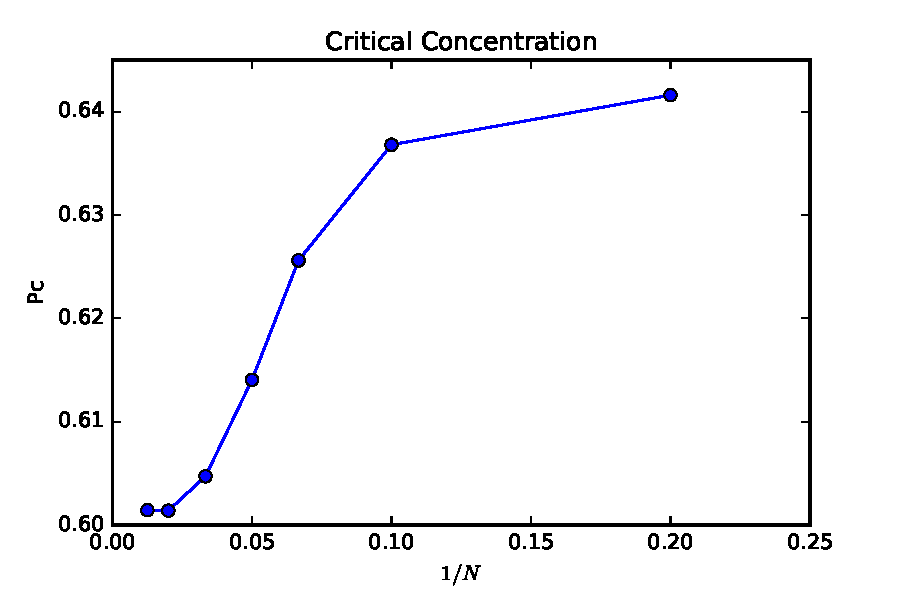
\includegraphics{Critical.pdf}
\end{figure}
According to the graph, we could extrapolate to the infinite size limit $p_c(0)\approx0.602$.
\section{(b)}
\end{document}
